\centering

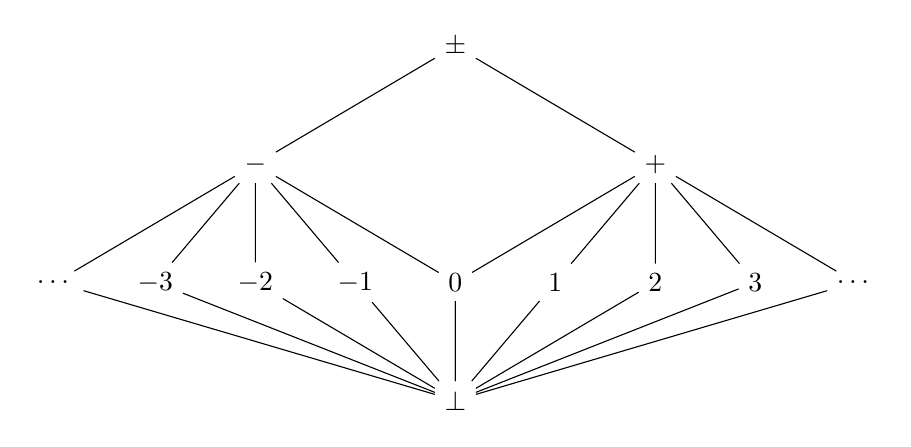
\begin{tikzpicture}[level 1/.style={sibling distance=2in},
                    level 2/.style={sibling distance=0.5in}]
  \node{$\pm$}
    child {node {$-$}
           child {node (-inf) {\ldots}}
           child foreach \x in {-3,...,-1} {node (\x) {$\x$}}
           child {node (0) {$0$}
                  child {node (bot) {$\bot$}}}}
    child {node (+) {$+$}
           child[missing]
           child foreach \x in {1,...,3} {node (\x) {$\x$}}
           child {node (+inf) {\ldots}}};
    \draw (+) -- (0);
    \draw (bot) -- (-inf);
    \foreach \x in {-3,...,3} \draw (bot) -- (\x);
    \draw (bot) -- (+inf);
\end{tikzpicture}

\caption{Abstract interpretation over signs}
